\section{Численное моделирование математической модели пневмопривода с дискретными распределителями}

На основе проведенного в предыдущем разделе теоретического анализа, обобщим полученные
результаты в виде целостной математической модели пневмопривода с дискретными распределителями.
Полная математическая модель представляет собой систему из 9 дифференциальных уравнений:

\begin{equation}
	\begin{cases}
		\begin{aligned}
			M\ddot{x}                    & = p_1F_1 - p_2F_2 - p_\text{атм}(F_1 - F_2) - R_\text{тр}(\dot{x}) - R_\text{упор}(x,\dot{x});                   \\
			\frac{dp_1}{dt}              & = \frac{\gamma}{V_1(x)}\left(RT_1(G_{1\text{вх}} - G_{1\text{вых}}) - p_1 F_1\frac{dx}{dt}\right);               \\
			\frac{dp_2}{dt}              & = \frac{\gamma}{V_2(x)}\left(RT_2(G_{2\text{вх}} - G_{2\text{вых}}) + p_2 F_2\frac{dx}{dt}\right);               \\
			\frac{dT_1}{dt}              & = \frac{T_1}{p_1}\frac{dp_1}{dt} + \frac{(\gamma-1)T_1}{V_1(x)}\frac{dV_1}{dt};                                  \\
			\frac{dT_2}{dt}              & = \frac{T_2}{p_2}\frac{dp_2}{dt} + \frac{(\gamma-1)T_2}{V_2(x)}\frac{dV_2}{dt};                                  \\
			\frac{dz}{dt}                & = \dot{x} - \frac{\sigma_0|\dot{x}|}{g(\dot{x})}z;                                                               \\
			R_\text{упор}                & = \begin{cases}
				                                 k_\text{упор}(x - x_\text{мин}) + b_\text{упор}\dot{x},  & \text{если } x < x_\text{мин} ;                      \\
				                                 0,                                                       & \text{если } x_\text{мин} \leq x \leq x_\text{макс}; \\
				                                 k_\text{упор}(x - x_\text{макс}) + b_\text{упор}\dot{x}, & \text{если } x > x_\text{макс};
			                                 \end{cases} \\
			\tau_1 \frac{du_1}{dt} + u_1 & = u_{1\text{зад}};                                                                                               \\
			\tau_2 \frac{du_2}{dt} + u_2 & = u_{2\text{зад}};                                                                                               \\
			\tau_3 \frac{du_3}{dt} + u_3 & = u_{3\text{зад}};                                                                                              \\
			\tau_4 \frac{du_4}{dt} + u_4 & = u_{4\text{зад}}.                                                                                               \\
		\end{aligned}
	\end{cases}
	\label{eq:ch2/complete_model}
\end{equation}

Уравнение механического движения штока пневмоцилиндра выведено в разделе~\ref{sec:ch1/sec2} и учитывает силы от
воздействия давлений в полостях, силы трения и реакцию упоров. Сила трения $R_\text{тр}(\dot{x})$ определяется
по модели LuGre согласно уравнению~\eqref{eq:ch2/friction_force},
с функцией Штрибека $g(\dot{x})$, заданной выражением~\eqref{eq:ch2/stiction_function}.

Уравнения изменения давлений в полостях пневмоцилиндра выведены в соответствии с уравнением~\eqref{eq:ch2/final_pressure_system}, а уравнения изменения
температур определяются выражениями из системы~\eqref{eq:ch2/energy_balance_final}.

Массовые расходы через распределители выражаются согласно уравнениям~\eqref{eq:ch2/mass_flow}

Последние четыре уравнения в системе~\eqref{eq:ch2/complete_model} описывают динамику переключения распределителей в соответствии с управляющими сигналами $u_{i\text{зад}}$,
формируемыми системой управления. Дифференциальные уравнения первого порядка для переключения соответствуют ~\eqref{eq:ch2/switching_dynamics}.

Ключевым элементом системы является блок управления, формирующий управляющие
воздействия на дискретные распределители. В обобщенном виде алгоритм управления может быть представлен как:

\begin{equation}
	[u_{1\text{зад}}, u_{2\text{зад}}, u_{3\text{зад}}, u_{4\text{зад}}] = F(x_\text{зад}, x, \dot{x}, p_1, p_2, t),
	\label{eq:ch2/control_generic}
\end{equation}
где $F$ -- функция управления, реализующая конкретный алгоритм;
$x_\text{зад}$ -- заданное положение штока пневмоцилиндра, $t$ -- текущее время.
\nomenclature{$x_\text{зад}$}{Заданное положение штока пневмоцилиндра\nomrefeqpage}
\nomenclature{$t$}{Текущее время\nomrefeqpage}
\nomenclature{$F$}{Функция управления\nomrefeqpage}

Важной особенностью разработанной математической модели является возможность интеграции различных алгоритмов
управления при сохранении общей структуры модели. В дальнейших разделах будут рассмотрены ПИД-регулятор с широтно-импульсной
модуляцией (ШИМ), многорежимное управление в скользящих режимах (УСР), нечеткое управление и прогнозное управление (MPC).

Каждый из этих алгоритмов реализует свой вариант функции $F$ в уравнении \eqref{eq:ch2/control_generic}, определяя
специфическую логику переключения распределителей для достижения заданного положения штока.

Для численного решения системы дифференциальных уравнений \eqref{eq:ch2/complete_model} использован метод обратных
дифференциальных формул (BDF) с переменным порядком и адаптивным шагом. Данный метод особенно эффективен для
решения жестких систем благодаря своей высокой устойчивости, при этом обеспечивая необходимую точность.
Основные параметры численного интегрирования выбраны согласно таблице~\ref{tab:params}.

\begin{table}[h]
	\centering
	\caption{Параметры интегрирования}
	\begin{tabular}{ll}
		\midrule
		\textbf{Параметр}                                    & \textbf{Значение} \\
		\midrule
		Относительная погрешность ($\varepsilon_\text{rel}$) & $10^{-6}$         \\
		Абсолютная погрешность ($\varepsilon_\text{abs}$)    & $10^{-8}$         \\
		Начальный шаг интегрирования ($h_0$)                 & $10^{-5}$ с       \\
		Максимальный шаг интегрирования ($h_\text{max}$)     & $10^{-3}$ с       \\
		\midrule
	\end{tabular}
	\label{tab:params}
\end{table}

Программная реализация математической модели построена по модульному принципу с использованием объектно-ориентированного подхода при помощи языка программирования Python.
Основные модули включают: пневмоцилиндр (реализует уравнения движения и термодинамические процессы), модуль трения (модель LuGre),
модуль распределителей (расчет массовых расходов), модуль управления (различные алгоритмы),
модуль решателя (численное интегрирование) и модуль визуализации.
Такая архитектура обеспечивает гибкость при исследовании различных алгоритмов управления. Схема программы представлена на рисунке~\ref{fig:ch2/architecture}.

\begin{figure}[h]
	\centering
	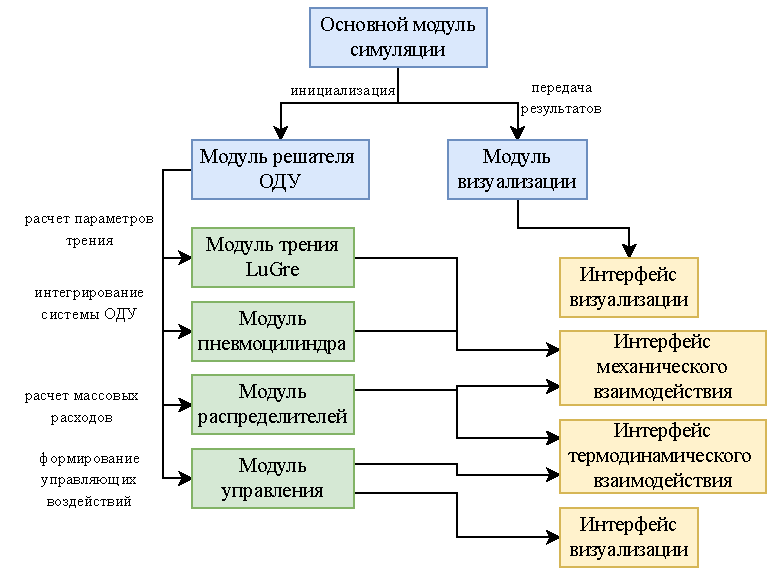
\includegraphics[width=1\textwidth]{part2/pneumatic_drive_architecture.pdf}
	\caption{Архитектура программы}
	\label{fig:ch2/architecture}
\end{figure}
